\documentclass[11pt]{article}

\usepackage{../handout}
\usepackage{graphicx}

% Side margins:
% Actual margin is 1 in + this number
\oddsidemargin -0.25in
\evensidemargin -0.25in

% Text width:
\textwidth 6.9in

% Top margin:
% Actual margin is 1.5 in + this number
\topmargin -.3in

% Text height:
\textheight 8.7in

% Handout Numbers

\newcommand{\PAOneNum}{1}
\newcommand{\WAOneNum}{2}
\newcommand{\PATwoNum}{3}
\newcommand{\PAThreeNum}{4}
\newcommand{\WATwoNum}{5}
\newcommand{\WATwoSolNum}{6}
\newcommand{\WAOneSolNum}{7}
\newcommand{\WAThreeNum}{8}
\newcommand{\WAFourNum}{9}
\newcommand{\WAThreeSolNum}{10}
\newcommand{\PAFourNum}{11}
\newcommand{\WAFourSolNum}{12}
\newcommand{\WAFiveNum}{13}
\newcommand{\WAFiveSolNum}{14}
\newcommand{\WASixNum}{15}
\newcommand{\WASixSolNum}{16}
\newcommand{\PAFiveNum}{17}
\newcommand{\WASevenNum}{18}
\newcommand{\WASevenSolNum}{19}
\newcommand{\PAExtraNum}{20}
\newcommand{\WAEightNum}{21}
\newcommand{\WAEightSolNum}{22}
\newcommand{\PASixNum}{23}
\newcommand{\WANineNum}{24}
\newcommand{\WANineSolNum}{25}
\newcommand{\WATenNum}{26}
\newcommand{\WATenSolNum}{27}
\newcommand{\WAElevenNum}{28}
\newcommand{\WAElevenSolNum}{29}


\begin{document}
\handout{\WAOneNum}{2}{Written Assignment 1 \\ Due October 9 at 5:00 PM}

This assignment asks you to prepare written answers to questions on regular
languages and finite automata. Each of the questions has a short answer. You
may discuss this assignment with other students and work on the problems
together, however, your write-up must be your own individual work.  Remember
that written assignments are to be turned in either at the start of lecture, 
electronically, or in the CS143 homework box outside Gates 411 by 5:00 PM on the due date.

\bigskip

\begin{enumerate}
	% #1
	\item 
	Give a DFA for each of the following languages over the alphabet $\Sigma = \{a,b\}$. 
	\begin{itemize}
		\item $L_1$: \emph{All strings that contain at least two a's} 
		\item $L_2$: \emph{All strings that contain at least one b} 
		\item $L_3$: \emph{All strings that contain at least two a's and at least one b} 
		\item $L_4$: \emph{All strings that contain at most one a or no b's} 
	\end{itemize}
	
	{\bf Aside}: This example illustrates that regular
	languages are closed under intersection and complementation. Note that
	$L_3 = L_1 \cap L_2$ and $L_4 = \Sigma^{*} - L_3$, where $\Sigma^{*}$
	represents the language containing all strings over the alphabet $\Sigma$. 
	
	% #2
	\item Let $\Sigma_m = \{ a_1,\ldots,a_m \}$ be an alphabet containing $m$
	elements, for some integer $m \geq 1$.  Let $L_m$ be the following
	language that includes all strings in which at least one of the characters
	occurs an even number of times, i.e.
	\begin{center}
		\emph{All strings in which} $a_i$ \emph{occurs an even number of times for
			some} $i$, \emph{where} $1 \leq i \leq m$
	\end{center}
	The following figure shows an NFA for the language $L_2$. 
	\begin{center}
		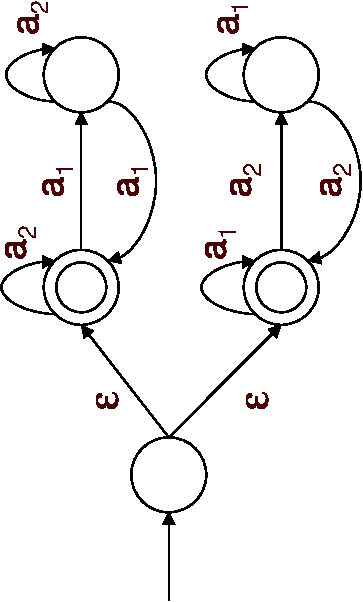
\includegraphics[height=2.3in,angle=-90]{wa1-q2.pdf}
	\end{center}
	Construct a DFA for the language $L_2$. Also construct an NFA for the
	language $L_3$.
	\medskip \\
	{\bf Aside:}
	Non-deterministic finite automata (NFAs) are no more powerful than
	DFAs in terms of the languages that they can describe.  However, NFAs can
	be exponentially more succinct than DFAs, as this problem
	demonstrates. 
	For the language $L_m$, there exists an NFA of size at most $2m+1$  while any
	DFA must have size at least $2^m$. Note that the 
	DFA for the language $L_3$ is not as easy to construct as the NFA for
	the language $L_3$. 
	
	\newpage
	
	% #3
	\item Write regular expressions for the following languages over the 
		alphabet $\Sigma = \{0,1\}$:
	\begin{enumerate}
		\item All strings that contain at least one 0 and at least one 1 and that also 
			end with at least two 1s.
		\item All strings that do not begin with 01.
		\item All strings that contain an odd number of 1s.
		\item All strings that contain exactly two 1s and at least one 0.
	\end{enumerate}
	
	% #4
	\item Give a one-sentence description and a regular expression 
	      for the language over the alphabet $\Sigma = \{0,1\}$ described
	      by the following deterministic finite automaton (DFA):
	\begin{center}
		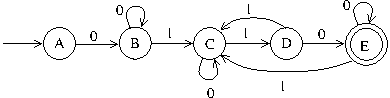
\includegraphics{wa1-q4.pdf}
	\end{center}
	
	% #5
	\item For each of the following lexical specifications, give a regular expression 
		describing the language of possible outputs. Assume that all inputs are strings 
		of 0s and 1s only.
	\begin{enumerate}
		\item Specification 1:
			\begin{verbatim}
			0       { print ("c"); }
			00      { print ("a"); }
			1       { print ("b"); }
			\end{verbatim}
			
		\item Specification 2:
			\begin{verbatim}
				(0+)(1+) { print("a"); }
				0        { print("b"); }
				1        { print("c"); }
			\end{verbatim}
	\end{enumerate}
	
\end{enumerate}
\end{document}
